\documentclass[letterpaper, 10 pt, conference]{ieeeconf}

\overrideIEEEmargins
\usepackage[pdftex]{graphicx}

\title{\LARGE \bf A Survey of Graph Mining}
\author{Andy Malinsky}% <-this % stops a space

\begin{document}
\maketitle
\thispagestyle{empty}
\pagestyle{empty}

\section{INTRODUCTION}
In modern society, the boom of technology has resulted in an exponential stream of data, or Big Data. Every day more than 2.5 quintillion bytes of data are created \cite{c10}. The main challenges of Big Data include volume, variety, velocity, variability, and value \cite{c9}. Knowing how to take that data and analyze it is a crucial part of understanding relationships in the world. In order to discover patterns and relationships within large data sets, research scientists are using the process of data mining. By employing different data mining techniques, the challenge of handling Big Data becomes more manageable. One of these key data mining techniques is called graph mining. Graph mining is an important research area, because it allows for the extraction of patterns from graph structures. Some applications include the analysis of social networks, Web graphs, spatial networks, and bioinformatics \cite{c1}. Graph mining approaches may be based on classification, clustering, or decision trees data mining techniques \cite{c7}. The figure below depicts a type of graph that would be useful for data analytics.

\begin{figure}[ht!] %!t
\centering
\hspace*{-4cm} 
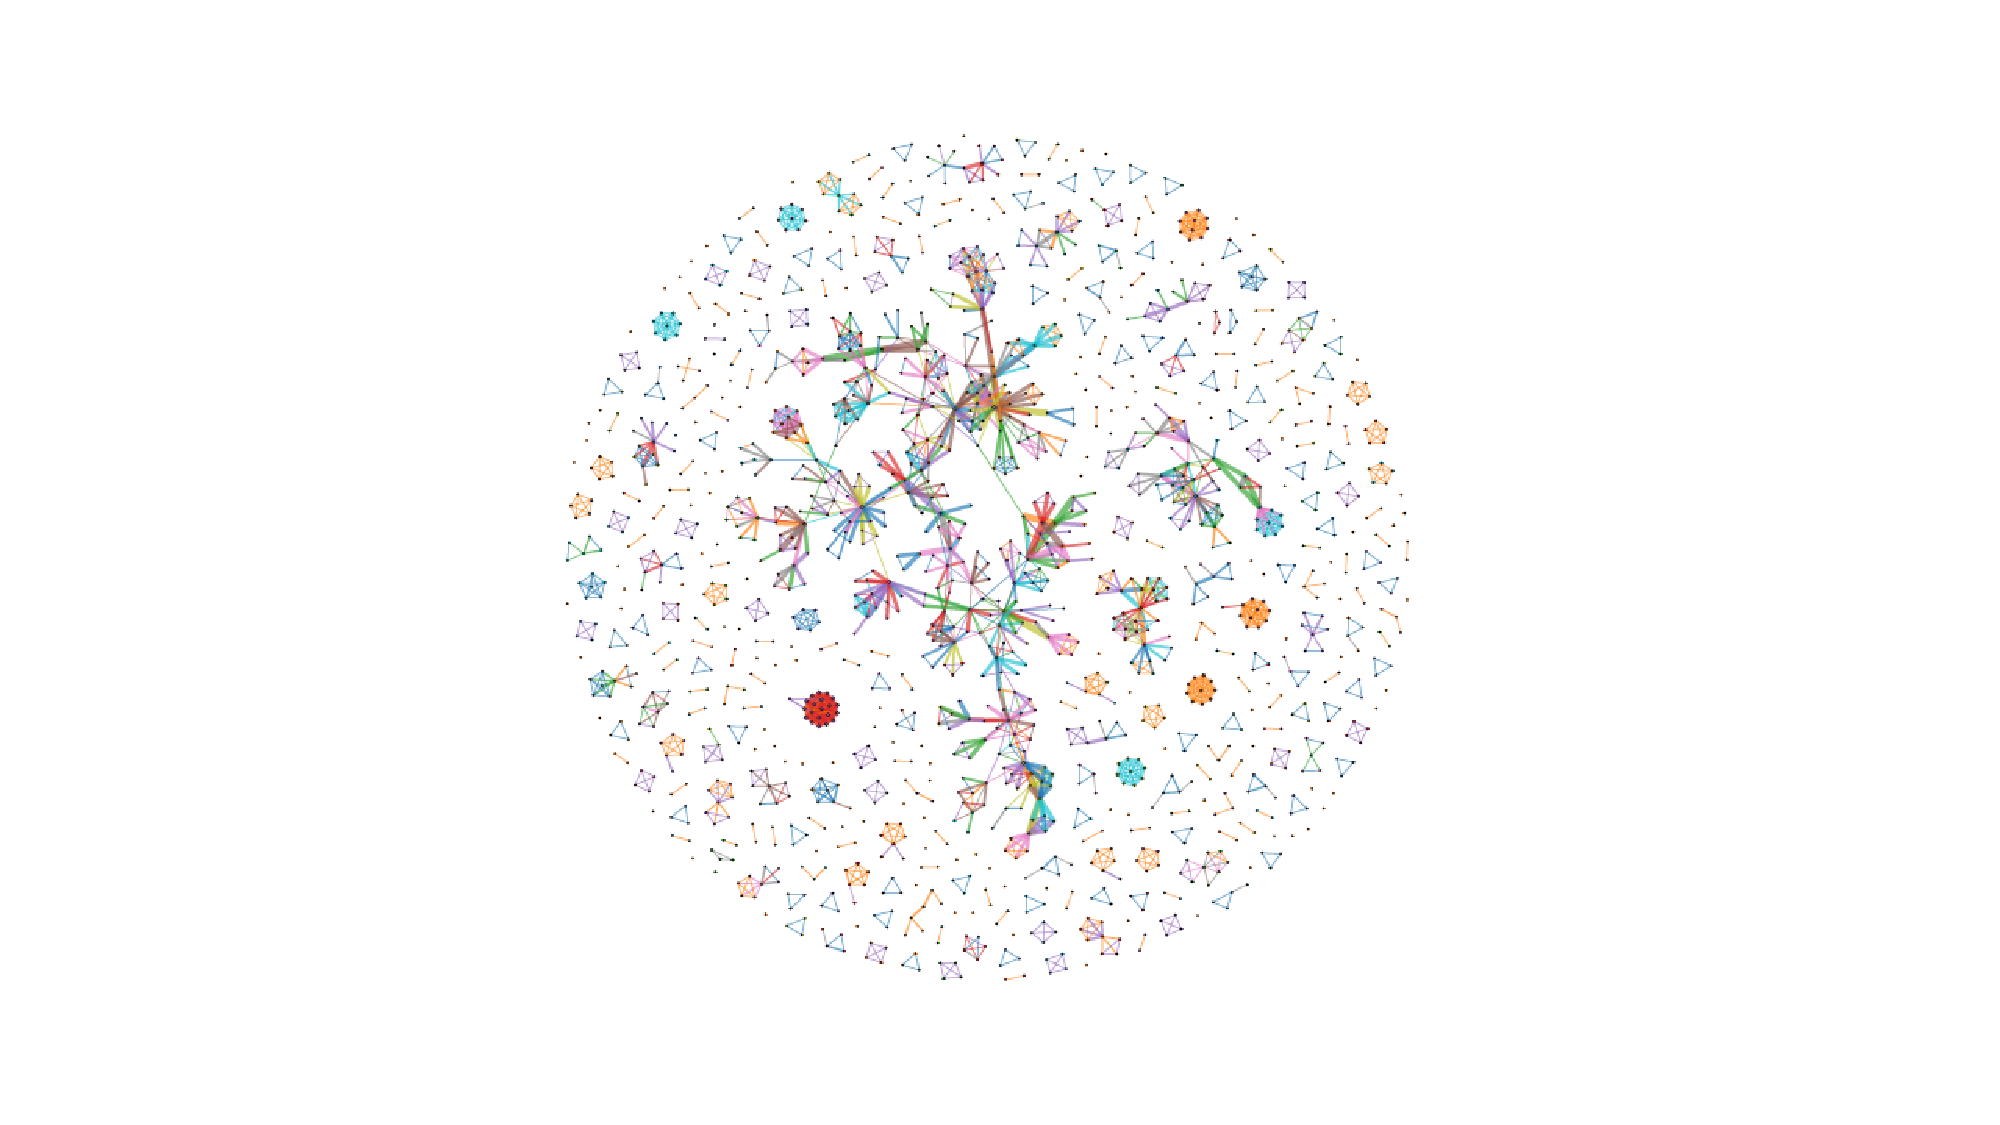
\includegraphics[height=3.5in]{f1.pdf}
\caption{This is an example of a graph created by the visual analytics tool GRAPHVIS \cite{c11}. Graphs provide opportunities to explore visualizations of data. This can make it easier to perform interactive analysis and make it possible to present obtained patterns and relationships. Connections between nodes along edges allow for clustering algorithms to predict clusters of similar data.}
\label{graph_example}
\end{figure}

Obtaining or recognizing patterns within graphs is the research problem of graph mining. In this paper I will discuss different graph mining techniques, methods, and algorithms utilized by a select few examples in the field in recent years.

\hfill
\section{LITERATURE REVIEW}

\subsection{Arabesque}
One novel graph mining approach that presented in recent years is known as Arabesque \cite{c2}. The development and design of graph mining algorithms is a current challenging area of research. In an effort toward providing a solution to graph mining problems, they proposed Arabesque, "the first embedding exploration system specifically designed for distributed graph mining". By taking inputs that are graph structures, or have labeled nodes and edges, the algorithm can seek connected graph patterns through exploration of subgraphs. They have constructed an API that enables users to process such graph inputs. Contributions they made include proposing embedding exploration as a useful tool for graph mining and demonstrate scalability of distributed techniques. Their novel graph mining framework Arabesque focuses on a simple API and a scalable distributed graph mining algorithm, and provides another option for data analysis. 

\hfill
\subsection{SNAP}
The Stanford Network Analysis Platform (SNAP), is a general purpose and high performance system that provides easy-to-use high-level operations for analysis and manipulation of large networks \cite{c3}. SNAP serves as a graph mining library that utilizes network analysis algorithms to process through the nodes and edges of a graph structure. At the core of the system are classes labeled as \emph{graph and network containers}. Three \emph{graph methods} of generation, manipulation, and analytics provide different tools for the user's specific tasks for either the graph or network container. This allows for a streamlined experience. At a lower level, a graph in SNAP is represented by a hash table of nodes in the graph, with vectors of adjacent nodes listed. The SNAP system is unique, because graph representation provides a balance between modifying graph structure and executing graph algorithms.

\hfill
\subsection{CATCHSYNC}
Another novel graph mining method is called CATCHSYNC \cite{c4}. This method was made in an effort to automatically detect suspicious behavior within a given network. Based off of nodes and edges, the method looks for synchronized or rare behavior. Applications of this type of analysis can be found in many places on the Internet. Threats such as botnets can cause trouble with web traffic to a particular website. This can result in a DDOS attack, or a distributed denial of service. Therefore, the goal of this algorithm is to attempt to detect artificial or fraudulent behavior by analyzing the patterns and dynamic relationships between nodes in a network or social graph. Results of the method prove to be scalable in linear time, parameter free, and side-information oblivious. In the paper, they tested the algorithm on social graphs of users on the online platforms of Twitter and Tencent Weibo. Three data sets ranging from one billion edges to twelve billion edges were experimented on. Their results showed outperformed other competitors in both fraud detection accuracy and speed.

\hfill
\subsection{Market Basket Analysis}
Market Basket Analysis (MBA) is a classic approach to gathering information from data in retail and department stores \cite{c5}. Traditional methods of analyzing this type of data include frequent item set discovery and K-means clustering. In an effort to avoid poor quality of output results, this paper develops a novel approach to MBA that utilizes graph mining techniques. The new method uses overlap communities which was shown to outperform the traditional methods. They construct a network representation out of transactional data and build an adjacency matrix for product-to-product weights. Their graph mining approach to MBA provides an option for extracting useful information from large data sets of product sales transactions.

\hfill
\subsection{People-to-People Matching}
Matching two distinct users within a given network is the goal for many social platforms \cite{c6}. Some real world examples of networks include job search, academic mentoring, marketplace transactions, and online dating. In order to define a successful match-making system the connections between users needs to be established. This paper utilizes Social Network Analysis (SNA), essentially a way to define and derive relationships among users. Several properties to consider when analyzing social networks include size, density, distributions, connected components and community structures. They conducted an in-depth study on an online dating social graph using SNA methods. Concluding results demonstrated that richer matches are identified through combining the attributes of the nodes and their dynamic interactions in the network.

\hfill
\subsection{Pattern Mining Applications}
The development of efficient pattern mining algorithms is a key problem in the context of graph mining techniques \cite{c8}. Graph patterns are derived in an effort to provide insight into real-world phenomena. One predominant application is in chemistry. Nodes can be made to represent atoms and edges made to represent the bonds between those atoms. Chemical compounds in their graph representations may be compared with other chemical compounds that are represented as a graph with edges and nodes. Also, the paper points out that biology is another domain where graph patterns are useful. Protein structures can be represented as a set of elements with nodes and edges. Then, a resulting graph would be a protein interaction network. This demonstrates implications for disease prevention and detection.

\begin{figure}[ht!] %!t
\centering
% \hspace*{-1cm} 
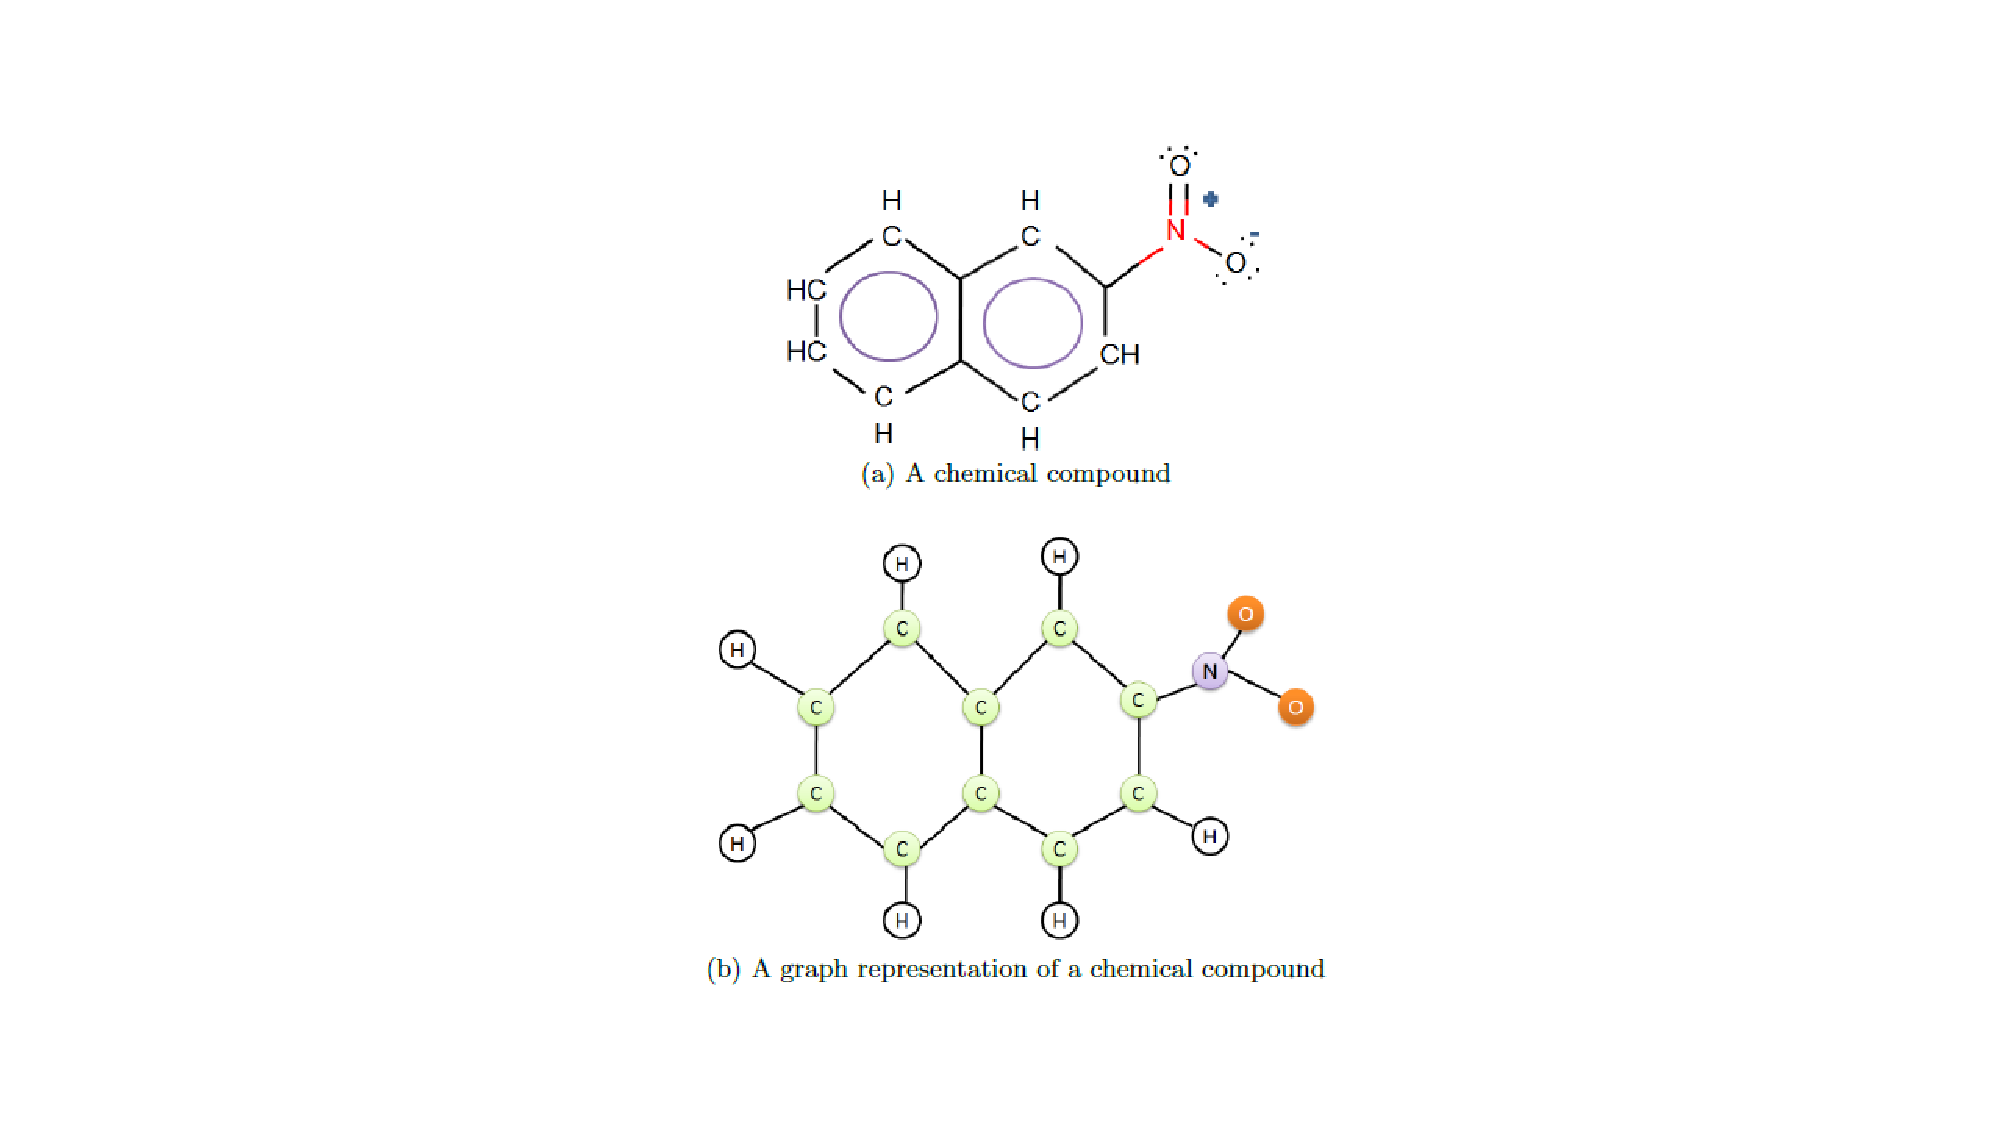
\includegraphics[height=5.5in, trim={10cm 0 0 0},clip]{f2.pdf}
\caption{These are examples of chemical compounds displayed in a graph representation\cite{c8}. By displaying molecules or compounds in such a manner, scientists and researchers are able to visualize the anatomical structures from another perspective. This also provides scientists a metric for comparing any two given chemical compounds. This method may then be used for data mining purposes such as classification or clustering. Similar compound structures may be more closely related and thus relationships in a network would offer respective insight.}
\label{graph_example_2}
\end{figure}

\hfill
\section{OPEN ISSUES AND FUTURE DIRECTIONS}
The trend one may notice about graph mining is that efficiency of pattern recognition is key. This may involve clustering, classification, or decision tree algorithms. However, the three aforementioned techniques may be considered traditional. Maybe novel algorithms or frameworks are needed to further remove the challenge of processing through infinitely larger data sets. Current methods seem to be working well with proven results, but a focus on further generalizing the pattern mining methods may be needed. Both accuracy and speed of results are factors in determining efficiency. The data mining technique of graph mining maintains the potential for providing key insights into the secrets hidden in our data.

\addtolength{\textheight}{-12cm}

\hfill
\begin{thebibliography}{99}

\bibitem{c1} Rehman, Saif Ur, Asmat Ullah Khan, and Simon Fong. "Graph mining: A survey of graph mining techniques." Seventh International Conference on Digital Information Management (ICDIM 2012). IEEE, 2012.
\bibitem{c2} Teixeira, Carlos HC, et al. "Arabesque: a system for distributed graph mining." Proceedings of the 25th Symposium on Operating Systems Principles. ACM, 2015.
\bibitem{c3} Leskovec, Jure, and Rok Sosič. "Snap: A general-purpose network analysis and graph-mining library." ACM Transactions on Intelligent Systems and Technology (TIST) 8.1 (2016): 1.
\bibitem{c4} Jiang, Meng, et al. "Catching synchronized behaviors in large networks: A graph mining approach." ACM Transactions on Knowledge Discovery from Data (TKDD) 10.4 (2016): 35.
\bibitem{c5} Videla-Cavieres, Ivan F., and Sebastian A. Rios. "Extending market basket analysis with graph mining techniques: A real case." Expert Systems with Applications 41.4 (2014): 1928-1936.
\bibitem{c6} Kutty, Sangeetha, Richi Nayak, and Lin Chen. "A people-to-people matching system using graph mining techniques." World Wide Web 17.3 (2014): 311-349.
\bibitem{c7} Rehman, Saif Ur, Asmat Ullah Khan, and Simon Fong. "Graph mining: A survey of graph mining techniques." Seventh International Conference on Digital Information Management (ICDIM 2012). IEEE, 2012.
\bibitem{c8} Aridhi, Sabeur, and Engelbert Mephu Nguifo. "Big graph mining: Frameworks and techniques." Big Data Research 6 (2016): 1-10.
\bibitem{c9} Fan, Wei, and Albert Bifet. "Mining big data: current status, and forecast to the future." ACM sIGKDD Explorations Newsletter 14.2 (2013): 1-5.
\bibitem{c10} Wu, Xindong, et al. "Data mining with big data." IEEE transactions on knowledge and data engineering 26.1 (2014): 97-107.
\bibitem{c11} Ahmed, Nesreen Kamel, and Ryan Anthony Rossi. "Interactive visual graph analytics on the web." Ninth International AAAI Conference on Web and Social Media. 2015.

\end{thebibliography}
\end{document}